\documentclass{beamer}
\usepackage[utf8]{inputenc}
\usepackage{graphicx}
\author[Sowmya Vajjala]{Instructor: Sowmya Vajjala}

\title[LING 410X]{LING 410X: Language as Data}
\subtitle{Semester: Spring '18}

\date{20 March 2018}

\institute{Iowa State University, USA}
%%%%%%%%%%%%%%%%%%%%%%%%%%%

\begin{document}

\begin{frame}\titlepage
\end{frame}

\begin{frame}
\frametitle{Class Outline}
\begin{itemize}
\item Assignment 4 - brief discussion
\item Introduction to topic modeling
\item Assignment 5 description
\item This week and next week: discussion about topic modeling, and how to make our own models
\end{itemize} 
\end{frame}

\begin{frame}
\frametitle{Announcement}
\begin{itemize}
\item Thursday: No class, as I am at a conference and our talk is scheduled at the same time. But, there is an optional exercise, based on Chapter 13 in the textbook.
\end{itemize}
\end{frame}

\begin{frame}
\frametitle{Rest of the semester}
Macro Analysis of Texts:
\begin{enumerate}
\item Classification (Chapter 12) - This is what we discussed before the break
\item Topic modeling (Chapter 13) - this week and next
\item Clustering (Chapter 11) - When talking about visualization, after topic modeling
\end{enumerate}
\end{frame}

\begin{frame}
\frametitle{Assignment 4 Grading}
\begin{itemize}
\item First question: frequent words in the training and testing csv files - straight forward steps (everyone did this part well) \pause
\item Second question:
\begin{itemize}
\item More like a exploratory assignment. The tutorial works, I wanted you to try changing somethings in that procedure and see what happens.
\item My take on your submissions: I liked the ones which documented their experiences -e.g., what worked, what failed? did they manage to get better results? etc. 
\item The errors some of you saw when you tried to change the SVM algorithm to something else: Are they only in Windows? (some of you did not see this). One other possibility: memory limits.
\item I did not deduct any points for these errors - they are a part of the assignment! 
\end{itemize}
\item Where to go from there: Look for some publicly available classification dataset (there are many, I gave some links last time) and try to do classification.
\end{itemize}
\end{frame}

\begin{frame}
\frametitle{}
\Large Introduction to Topic Modeling
\end{frame}

\begin{frame}
\frametitle{What is topic modeling?}
\begin{itemize}
\item Topic Models are a group of algorithms which attempt to discover latent themes in large collections of documents.
\item They use statistical methods to analyze word usage in the texts to discover what "themes" run through them, how these themes connect to each other etc. \pause
\item Good thing about them: they do not expect us to provide any prior annotations/categories for texts. Topics will "emerge" from the analysis.
\item Bad thing: Lot of math behind it (but we do not have to understand the math to apply topic models) \pause
\item One of the most popular methods of analyzing unstructured text data. 
\end{itemize}
\end{frame}

\begin{frame}
\frametitle{Latent Dirichlet Allocation (LDA)}
\begin{itemize}
\item LDA is the simplest topic modeling algorithm
\item Intuitions: 
\begin{itemize}
\item each document is a mixture of multiple topics
\item each topic can be characterized by some set of keywords related to that topic. 
\item a keyword can exist in multiple topics with different degrees of importance.
\end{itemize}
\end{itemize}
\end{frame}

\begin{frame}
\frametitle{What does a Topic Model do?-1}
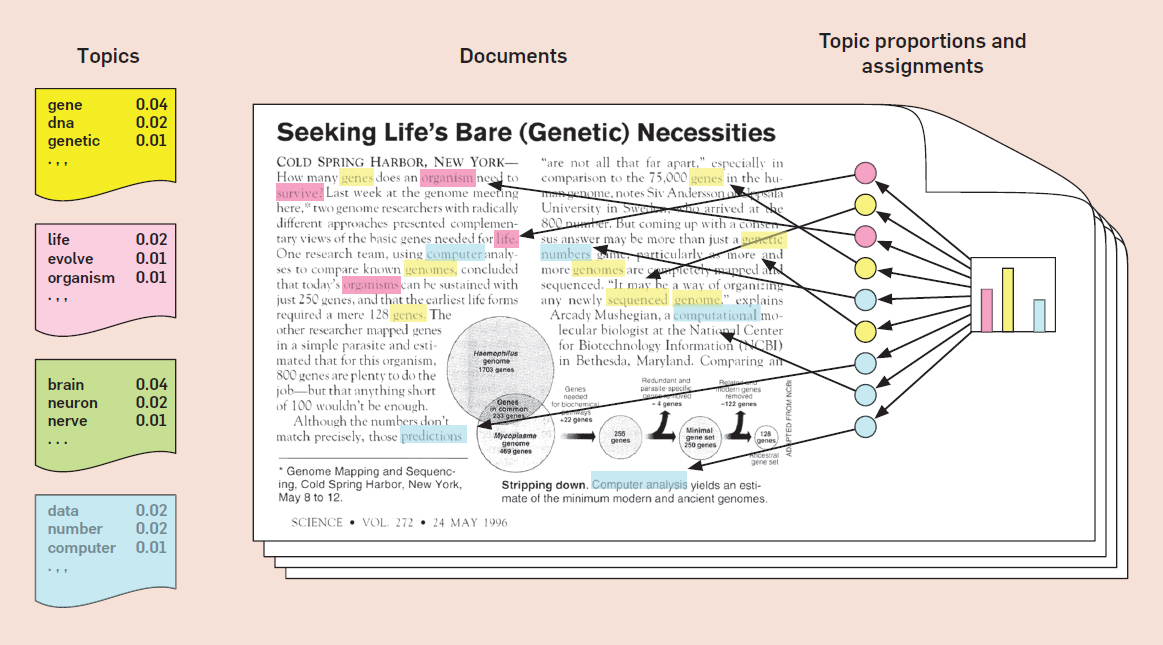
\includegraphics[width=0.9\textwidth]{topicmodelexample.jpg}
\footnotesize \\ source: \url{https://goo.gl/azc7Gc}
\end{frame}

\begin{frame}
\frametitle{What does a Topic Model do? -2}
Real inference with LDA - topic model built using 17000 articles from Science journal.
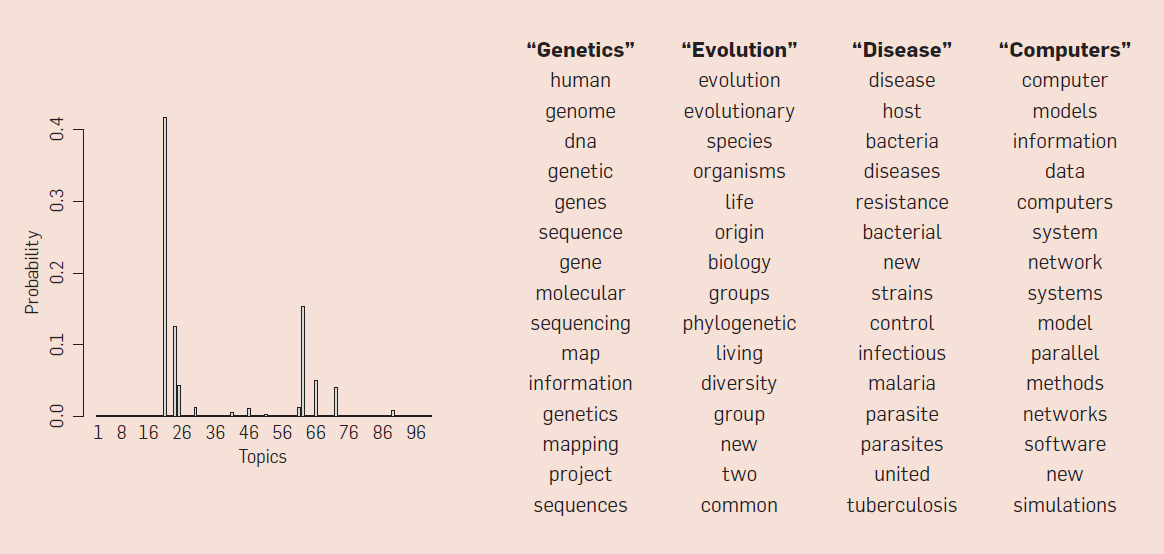
\includegraphics[width=0.9\textwidth]{topics2.jpeg}
\footnotesize \\ source: \url{https://goo.gl/azc7Gc}
\end{frame}

\begin{frame}
\frametitle{What does a Topic Model do? -3}
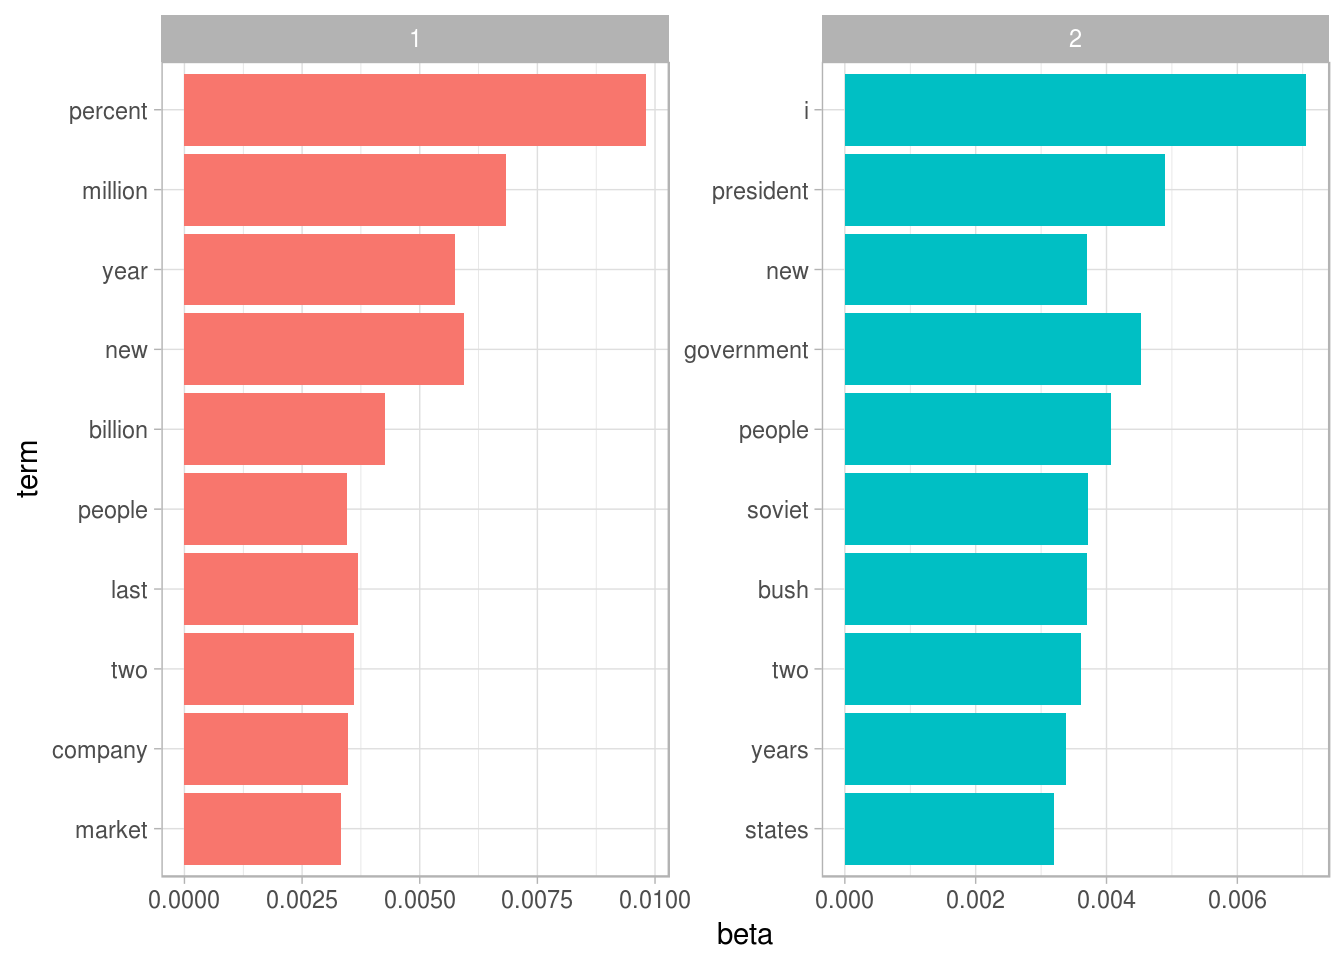
\includegraphics[width=0.7\textwidth]{tm-plot.png}
\footnotesize \\ source: \url{http://tidytextmining.com/topicmodeling.html}
\end{frame}

\begin{frame}
\frametitle{How are topic models useful? -1}
\framesubtitle{The bestseller code}
\begin{itemize}
\item One application comes from the textbook author.
\item He and his team analyzed best selling novels using topic models and concluded that best seller novels focus on a small number of topics instead of discussing 1000 things in one story :) 
\item Okay, it is more detailed than that, I am just telling a micro-summary of what they concluded.
\end{itemize}
\end{frame}

\begin{frame}
\frametitle{How are topic models useful?  -2}
\framesubtitle{Analysing topics over time}
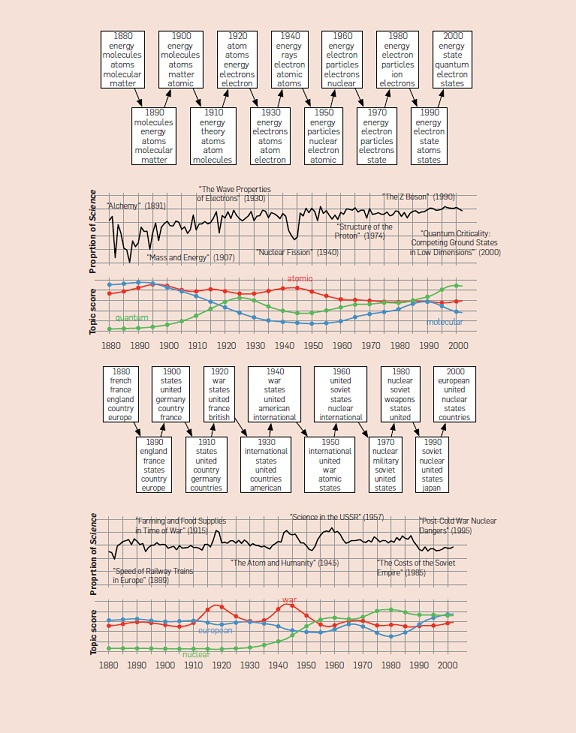
\includegraphics[width=0.6\textwidth]{topicmodels4.jpeg}
\footnotesize \\ source: \url{https://goo.gl/azc7Gc}
\end{frame}

\begin{frame}
\frametitle{How are topic models useful?  -3}
\framesubtitle{Analyzing topics by author}
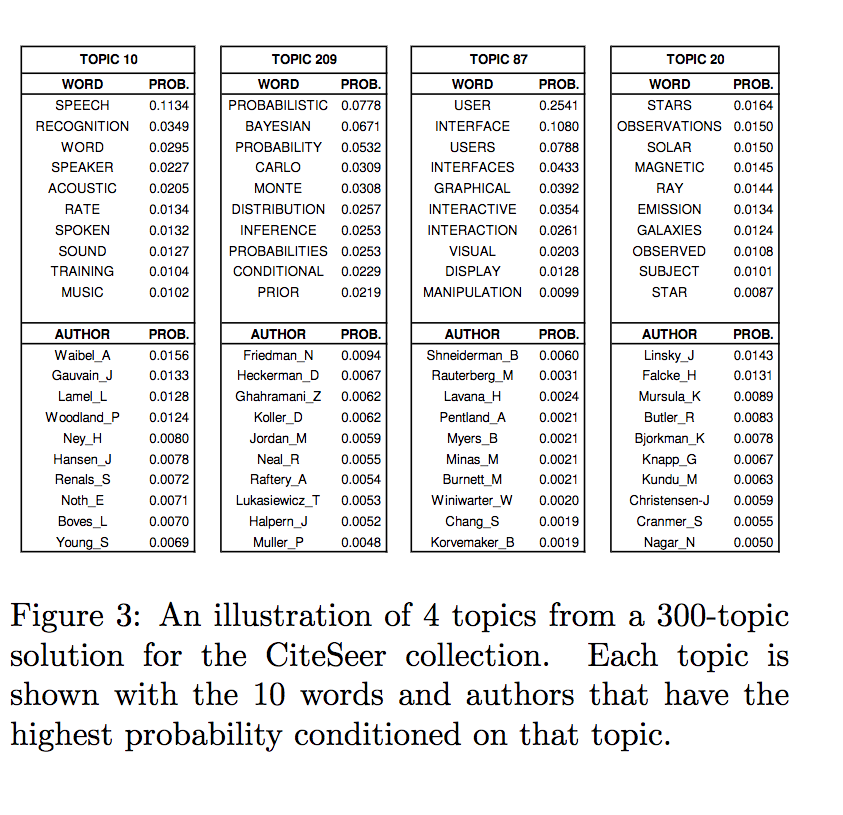
\includegraphics[width=0.7\textwidth]{topicmodels3.png}
\footnotesize \\ source: \url{https://mimno.infosci.cornell.edu/info6150/readings/398.pdf}
\end{frame}

\begin{frame}
\frametitle{How are topic models useful?  -4}
\framesubtitle{Picking up similar documents}
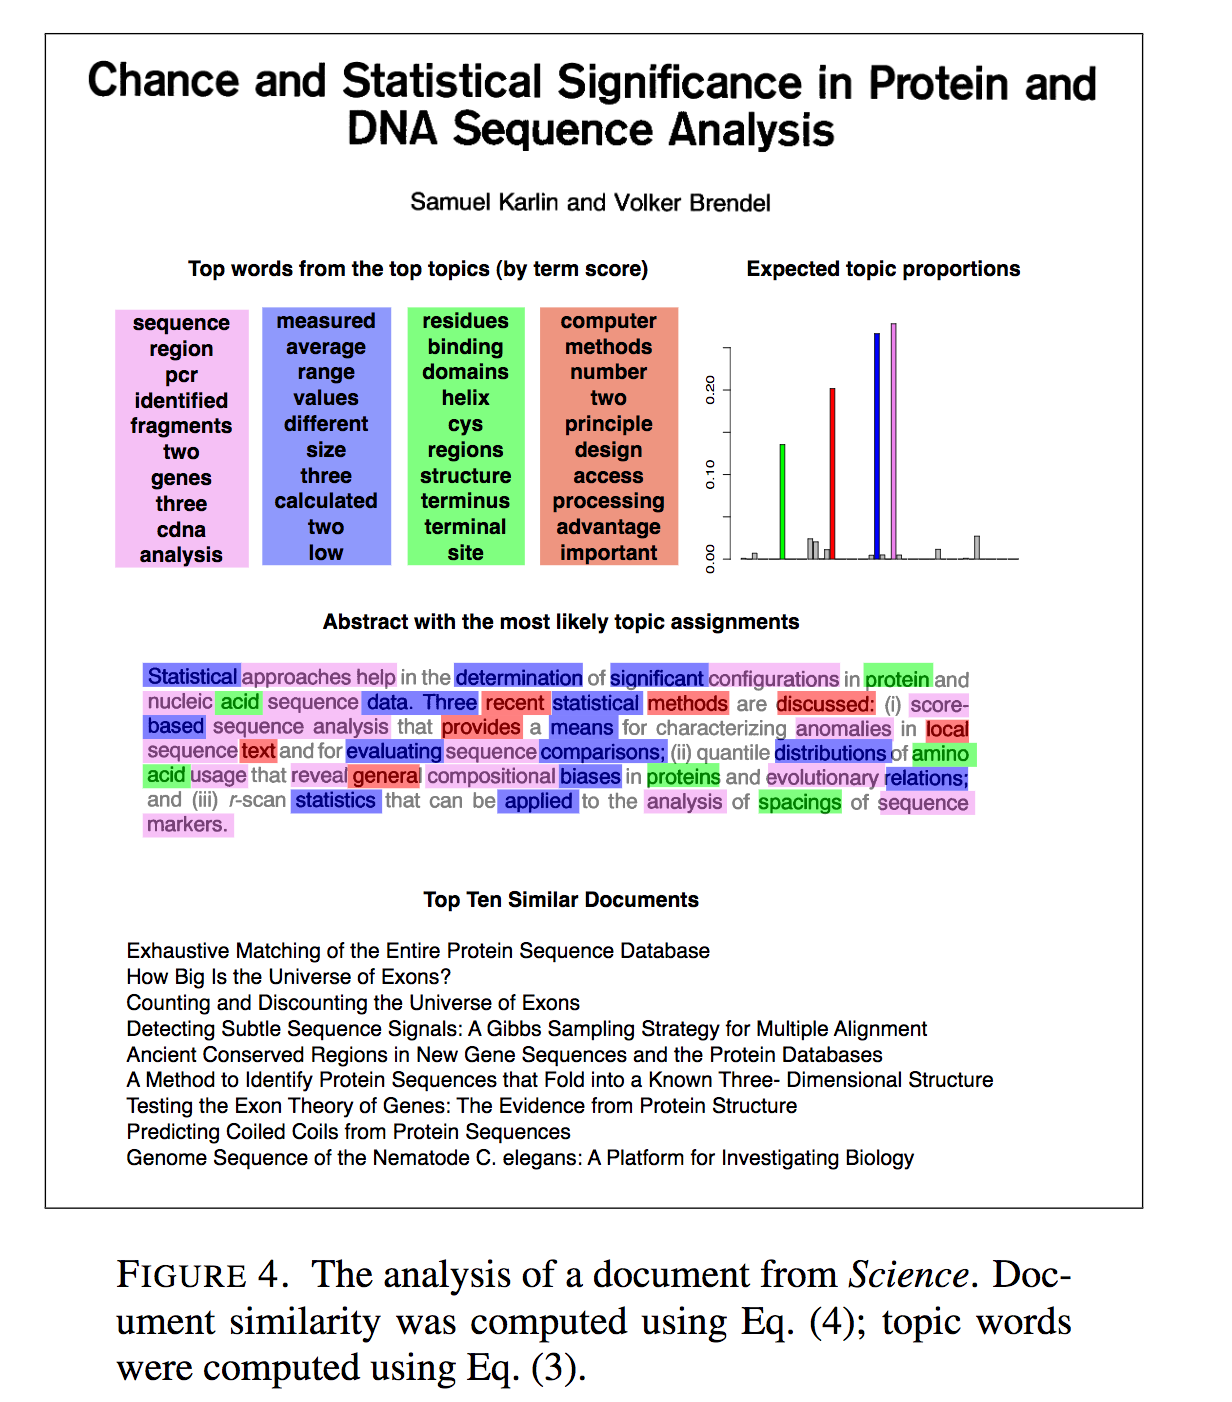
\includegraphics[width=0.6\textwidth]{topicmodels5.png}
\footnotesize \\ source: \url{http://www.cs.columbia.edu/~blei/papers/BleiLafferty2009.pdf}
\end{frame}

\begin{frame}
\frametitle{How are topic models useful?  -5}
\framesubtitle{Topic Graphs}
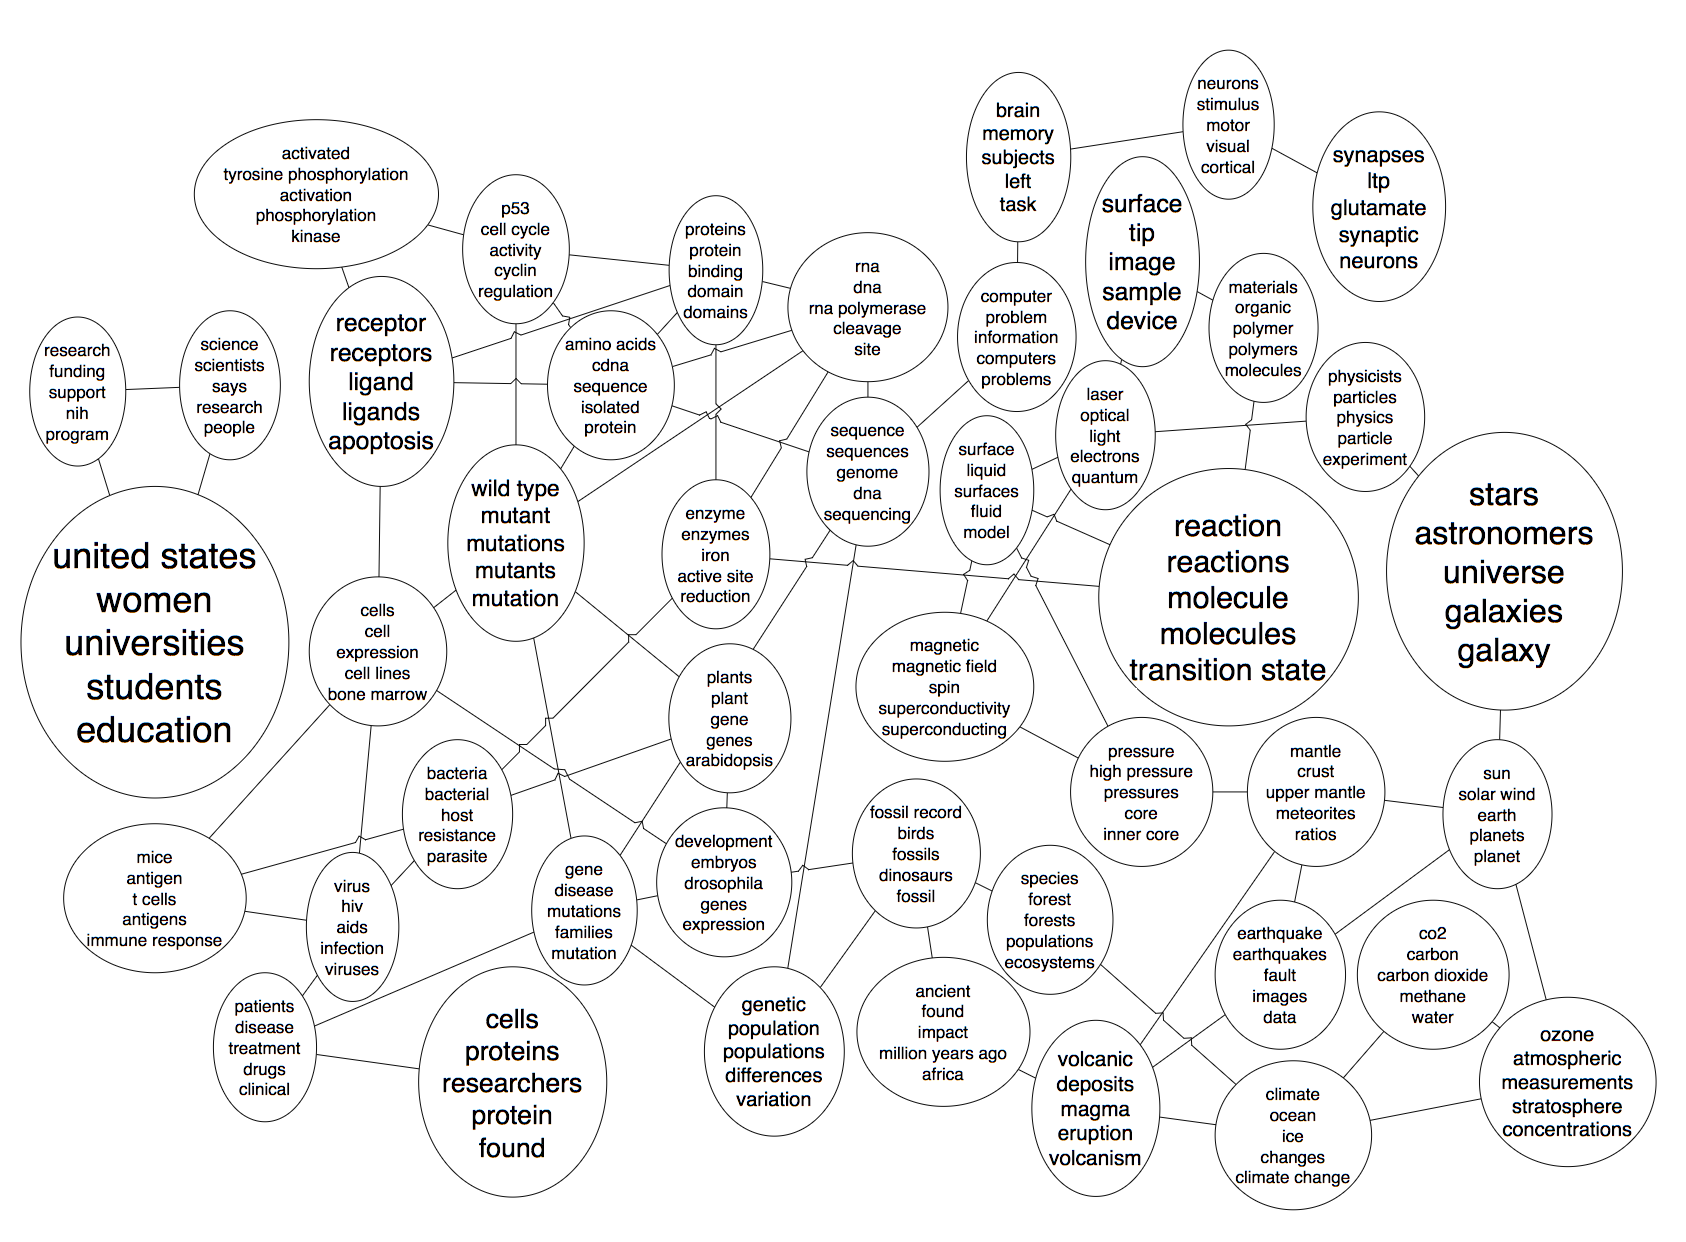
\includegraphics[width=0.7\textwidth]{topicgraph.png}
\footnotesize \\ source: \url{http://www.cs.columbia.edu/~blei/papers/BleiLafferty2009.pdf}
\end{frame}

\begin{frame}
\frametitle{Fun with topic models}
\url{https://gist.github.com/inkhorn/9044779\#file-recipe-analysis-r}
\end{frame}

\begin{frame}
\frametitle{A small exercise}
\begin{itemize}
\item Think for 5-10 minutes and try to list some (up to 5) applications of topic modeling in your discipline/topics of your interest
\item Now, discuss with our neighbor and compare your and their ideas
\item After about 15 minutes, let us discuss what you think are potential applications of topic models.
\end{itemize}
\end{frame}

\begin{frame}
\frametitle{Another small exercise}
\framesubtitle{Interpreting Topic Models}
What do you think of these topics (and their 5 most frequent keywords)? If you are asked to evaluate this topic model now, what will you look for? Think and discuss with your classmates for 5 minutes and we will later collect all answers. \small
\begin{itemize}
\item Topic 1 : Onion, Cream, Black pepper, Milk, Cinnamon
\item Topic 2: Cumin, Coriander, Turmeric, Fenugreek, Lemongrass
\item Topic 3: Vanilla, Cream, Almond, Coconut, Oat
\item Topic 4: Olive oil, tomato, parmesan cheese, lemon juice, garlic
\item Topic 5: soy sauce, scallion, sesame oil, cane molasses, roasted sesame seed
\item Topic 6: Milk, pepper, yeast, potato, lemon juice
\item Topic 7: Scallion, garlic, ginger, soy bean, pepper
\item Topic 8: Pepper, vinegar, onion, tomato, milk
\end{itemize}
\end{frame}

\begin{frame}
\frametitle{Some questions to ponder on:}
\begin{itemize}
\item Coherence among the keywords for a topic (Is some word looking out of place?)
\item Are there two topics that perhaps should be one?
\item Can we name the topics with what we think is the group?
\item Do you think the topic model learnt something about ingredients in this example? 
\end{itemize}
\end{frame}

\begin{frame}
\frametitle{Topic Models in R}
\begin{itemize}
\item different libraries: mallet, topicmodels, LDA etc.
\item Textbook follows mallet
\item Your Assignment 5 will use tm and topicmodels.
\end{itemize}
\end{frame}

\begin{frame}
\frametitle{Assignment 5 description}
\begin{itemize}
\item Deadline: 31st March
\item grade: 15\%
\item Num. questions: 1
\item What to do?: Build a topic model with the given data, following given instructions, and answer questions about what you did. 
\item Difficulty level: moderate, but the program takes a few minutes to complete running. 
\item R libraries needed: tm, topicmodels
\end{itemize}
\end{frame}

\begin{frame}
\frametitle{Topic Models - The Textbook Way}
\begin{itemize}
\item The author used mallet library to develop topic models for a corpus of novels and authors (same one he used in Chapters 11-12).
\item I will follow a different method (using tm, which we used before), but I recommend you to also go through this.
\item Note: You won't be an expert in text mining with one undergrad course. It is okay if you don't have a 100\% understanding of this.
\item The goal is to introduce you to different possible ways, give some ideas, and make you think.  
\end{itemize}
\end{frame}

\begin{frame}
\frametitle{For Thursday}
\begin{itemize}
\item I uploaded a Zip file, start with that. It contains all you need to follow Chapter 13's example.
\item Attendance question: Try to follow the textbook example (materials provided in a zip file), and write your notes in the forum for 22nd March. 
\end{itemize}
\end{frame}
%Brief description of topic models tutorial for thursday's class.

\begin{frame}
\frametitle{Next Week}
\begin{itemize}
\item Read this before coming to class: \url{https://goo.gl/L8MFfG}
\item Or this: \url{http://www.scottbot.net/HIAL/index.html@p=19113.html}
\item Optional, additional reading (for next week): \url{https://goo.gl/azc7Gc} (Has some math)
\item Other references: \url{http://tidytextmining.com/topicmodeling.html}
\item Attendance question for today: What are four things you need to build a topic model? - Answer can be found by reading first url. 
\end{itemize}
\end{frame}

\end{document}


\begin{frame}
\frametitle{Reports on final projects}
\begin{itemize}
\item Due date: 23rd March. 
\item Expectation: what problem will you solve? what is the data you will use?
\item What is the nature of the problem (classification, clustering, topic modeling, other analysis)?
\item How will you evaluate what you are doing?
\item What is your timeline for this?
\item What will you do if your plan of work does not work?
\end{itemize}
\end{frame}
